\section{Exercise 1}

Let $f(x) = \frac{1}{2}\sin(x) \1_{[0,\pi]}(x)$.
\begin{enumerate}
    \item For $n = 4$ \textbf{calculate} the first moment of the order statistic $X_{i:n}$ for every $i \in 1,\ldots, 4$.
    \item \textbf{Sketch a telling drawing} with the original density, the densities $f_{i:4}$ and $\E[X_{i:4}]$
\end{enumerate}

\subsection*{Solution Part 1}

In the first place, for $x \in [0,\pi]$
\[ \everymath{\displaystyle}
\arraycolsep=1.8pt\def\arraystretch{2.3}
\begin{array}{rrl}
    F(x) & = \frac{1}{2}\int_{-\infty}^{x}\sin(t)\1(t) dt & = \frac{1}{2}\int_{0}^{x}\sin(t) dt\\
    & = \cos(x) \Big|_{0}^x  & = \frac{1}{2}(1-\cos(x))\cdot \1_{[0,\pi]}(x)
\end{array} \]
Thus,
\[ \ol{F}(x) = \frac{1}{2}(1+\cos(x)) \cdot \1_{[0,\pi]}(x), \]
and,
\[ \everymath{\displaystyle}
\arraycolsep=1.8pt\def\arraystretch{1.8}
\begin{array}{rl}
    f_{i:n}(x) & = i \cdot \binom{n}{i} f(x) \cdot F^{i-1}(x) \cdot \ol{F}^{n-i}(x)\\
    & = i \cdot \binom{n}{i}\frac{1}{2^n} \cdot \sin(x) \cdot {(1-\cos(x))}^{i-1} \cdot {(1+\cos(x))}^{n-i}.
\end{array} \]
For simplicity, define $C_{i:n} = i \binom{n}{i}2^{-n}$. Now let $n = 4$. In order the calculate the exact expected value formula, we must use the following angle identities,

\[ \sin(x)\cos(x) = \frac{1}{2}\sin(2x),\hspace*{1em} \cos^2(x) = \frac{1}{2}(1+\cos(2x)), \]
and the result of these integrals
\[ \int x\sin(kx) dx = \frac{\sin(kx)-kx\cos(kx)}{k^2}.\]
From now on I'm going to simplify the trigonometric expressions using the TR8 algorithm provided by the \href{https://docs.sympy.org/latest/modules/simplify/fu.html#}{\underline{ package sympy}}. Also, use the package to integrate and evaluate the final expression. As always, the code is included with this document.


\begin{itemize}
    \item $\boldsymbol{i = 1:}$ 
    \[ C_{1:4}^{-1} \cdot f_{1:4} = \frac{7 \sin{\left(x \right)}}{4} + \frac{7 \sin{\left(2 x \right)}}{4} + \frac{3 \sin{\left(3 x \right)}}{4} + \frac{\sin{\left(4 x \right)}}{8},\]

    \[ C_{1:4}^{-1} \cdot \E[X_{1:4}] = C_{1:4}^{-1} \cdot \int_0^\pi x f_{1:4} dx.\]
    \[ = \everymath{\displaystyle}
    \arraycolsep=1.8pt\def\arraystretch{2.2}
    \begin{array}{r}
        - \frac{7 x \cos{\left(x \right)}}{4} - \frac{7 x \cos{\left(2 x \right)}}{8} - \frac{x \cos{\left(3 x \right)}}{4} - \frac{x \cos{\left(4 x \right)}}{32}\\
        \frac{7 \sin{\left(x \right)}}{4} + \frac{7 \sin{\left(2 x \right)}}{16} + \frac{\sin{\left(3 x \right)}}{12} + \frac{\sin{\left(4 x \right)}}{128}
    \end{array} \Bigg|_0^\pi = \frac{35 \pi}{32}. \]


    \item $\boldsymbol{i = 2:}$ 
    \[ C_{2:4}^{-1} \cdot f_{2:4} = \frac{3 \sin{\left(x \right)}}{4} + \frac{\sin{\left(2 x \right)}}{4} - \frac{\sin{\left(3 x \right)}}{4} - \frac{\sin{\left(4 x \right)}}{8},\]

    \[ C_{2:4}^{-1} \cdot \E[X_{2:4}] =  C_{2:4}^{-1} \cdot \int_0^\pi x f_{2:4} dx.\]
    \[ = \everymath{\displaystyle}
    \arraycolsep=1.8pt\def\arraystretch{2.2}
    \begin{array}{r}
        - \frac{3 x \cos{\left(x \right)}}{4} - \frac{x \cos{\left(2 x \right)}}{8} + \frac{x \cos{\left(3 x \right)}}{12} + \frac{x \cos{\left(4 x \right)}}{32}\\
        \frac{3 \sin{\left(x \right)}}{4} + \frac{\sin{\left(2 x \right)}}{16} - \frac{\sin{\left(3 x \right)}}{36} - \frac{\sin{\left(4 x \right)}}{128}
    \end{array} \Bigg|_0^\pi = \frac{55 \pi}{96}. \]


    \item $\boldsymbol{i = 3:}$
    \[ C_{3:4}^{-1} \cdot f_{3:4} = \frac{3 \sin{\left(x \right)}}{4} - \frac{\sin{\left(2 x \right)}}{4} - \frac{\sin{\left(3 x \right)}}{4} + \frac{\sin{\left(4 x \right)}}{8},\]

    \[ C_{3:4}^{-1} \cdot \E[X_{3:4}] = C_{3:4}^{-1} \cdot \int_0^\pi x f_{3:4} dx.\]
    \[ = \everymath{\displaystyle}
    \arraycolsep=1.8pt\def\arraystretch{2.2}
    \begin{array}{r}
        - \frac{3 x \cos{\left(x \right)}}{4} + \frac{x \cos{\left(2 x \right)}}{8} + \frac{x \cos{\left(3 x \right)}}{12} - \frac{x \cos{\left(4 x \right)}}{32}\\
        \frac{3 \sin{\left(x \right)}}{4} - \frac{\sin{\left(2 x \right)}}{16} - \frac{\sin{\left(3 x \right)}}{36} + \frac{\sin{\left(4 x \right)}}{128}
    \end{array} \Bigg|_0^\pi = \frac{73 \pi}{96}. \]

    \item $\boldsymbol{i = 4:}$
    \[ C_{4:4}^{-1} \cdot f_{4:4} = \frac{7 \sin{\left(x \right)}}{4} - \frac{7 \sin{\left(2 x \right)}}{4} + \frac{3 \sin{\left(3 x \right)}}{4} - \frac{\sin{\left(4 x \right)}}{8},\]

    \[ C_{4:4}^{-1} \cdot \E[X_{4:4}] = C_{4:4}^{-1} \cdot \int_0^\pi x f_{4:4} dx.\]
    \[ = \everymath{\displaystyle}
    \arraycolsep=1.8pt\def\arraystretch{2.2}
    \begin{array}{r}
        \- \frac{7 x \cos{\left(x \right)}}{4} + \frac{7 x \cos{\left(2 x \right)}}{8} - \frac{x \cos{\left(3 x \right)}}{4} + \frac{x \cos{\left(4 x \right)}}{32}\\
        \frac{7 \sin{\left(x \right)}}{4} - \frac{7 \sin{\left(2 x \right)}}{16} + \frac{\sin{\left(3 x \right)}}{12} - \frac{\sin{\left(4 x \right)}}{128}
    \end{array} \Bigg|_0^\pi = \frac{93 \pi}{32}. \]
\end{itemize}

Therefore,

\[ \E [X_{1:4}] = \frac{35 \pi}{128},\hspace*{1em} \E [X_{2:4}] = \frac{55 \pi}{128},\]
\[ \E [X_{3:4}] = \frac{73 \pi}{128},\hspace*{1em} \E [X_{4:4}] = \frac{93 \pi}{128}.\]

\subsection*{Solution Part 2}

\begin{figure}[h] % [h] stands for "here", you can use other options like [t] for top, [b] for bottom, [p] for page of floats
    \centering
    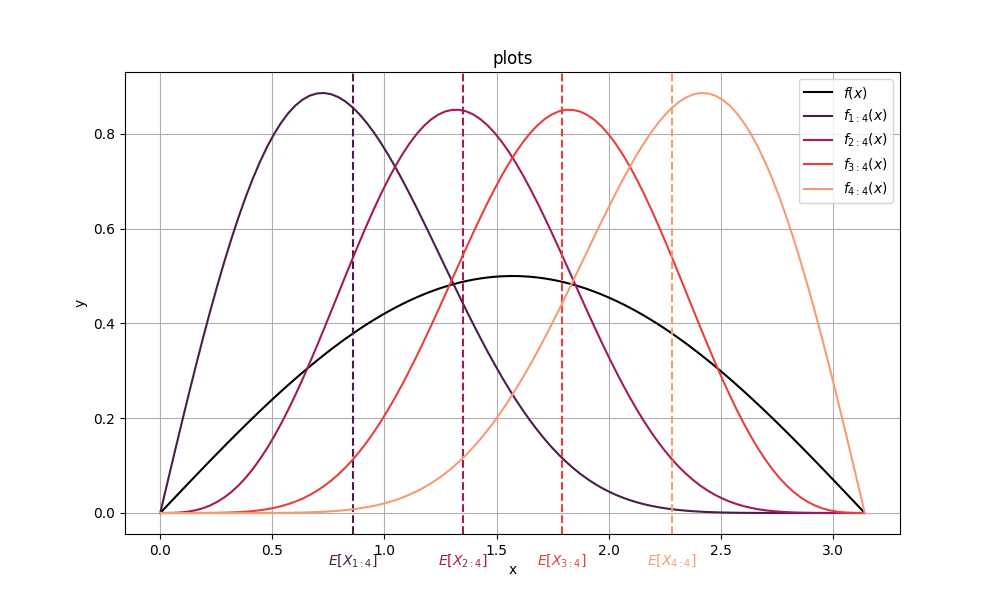
\includegraphics[width=0.9\textwidth]{../simulation/1b.png} % Change example-image to your image file name
    \caption{This is a floating figure with an image.}
    \label{fig:example}
\end{figure}

